% Important: If latex complains about unicode characters,
% please use "\usepackage[utf8x]{inputenc}" in your preamble
% You can change the size of the picture by putting it into the construct:
% 1) \resizebox{10cm}{!}{"below picture"} to scale horizontally to 10 cm
% 2) \resizebox{!}{15cm}{"below picture"} to scale vertically to 15 cm
% 3) \resizebox{10cm}{15cm}{"below picture"} a combination of above two
% It is not recomended to use the scale option of the tikzpicture environment.
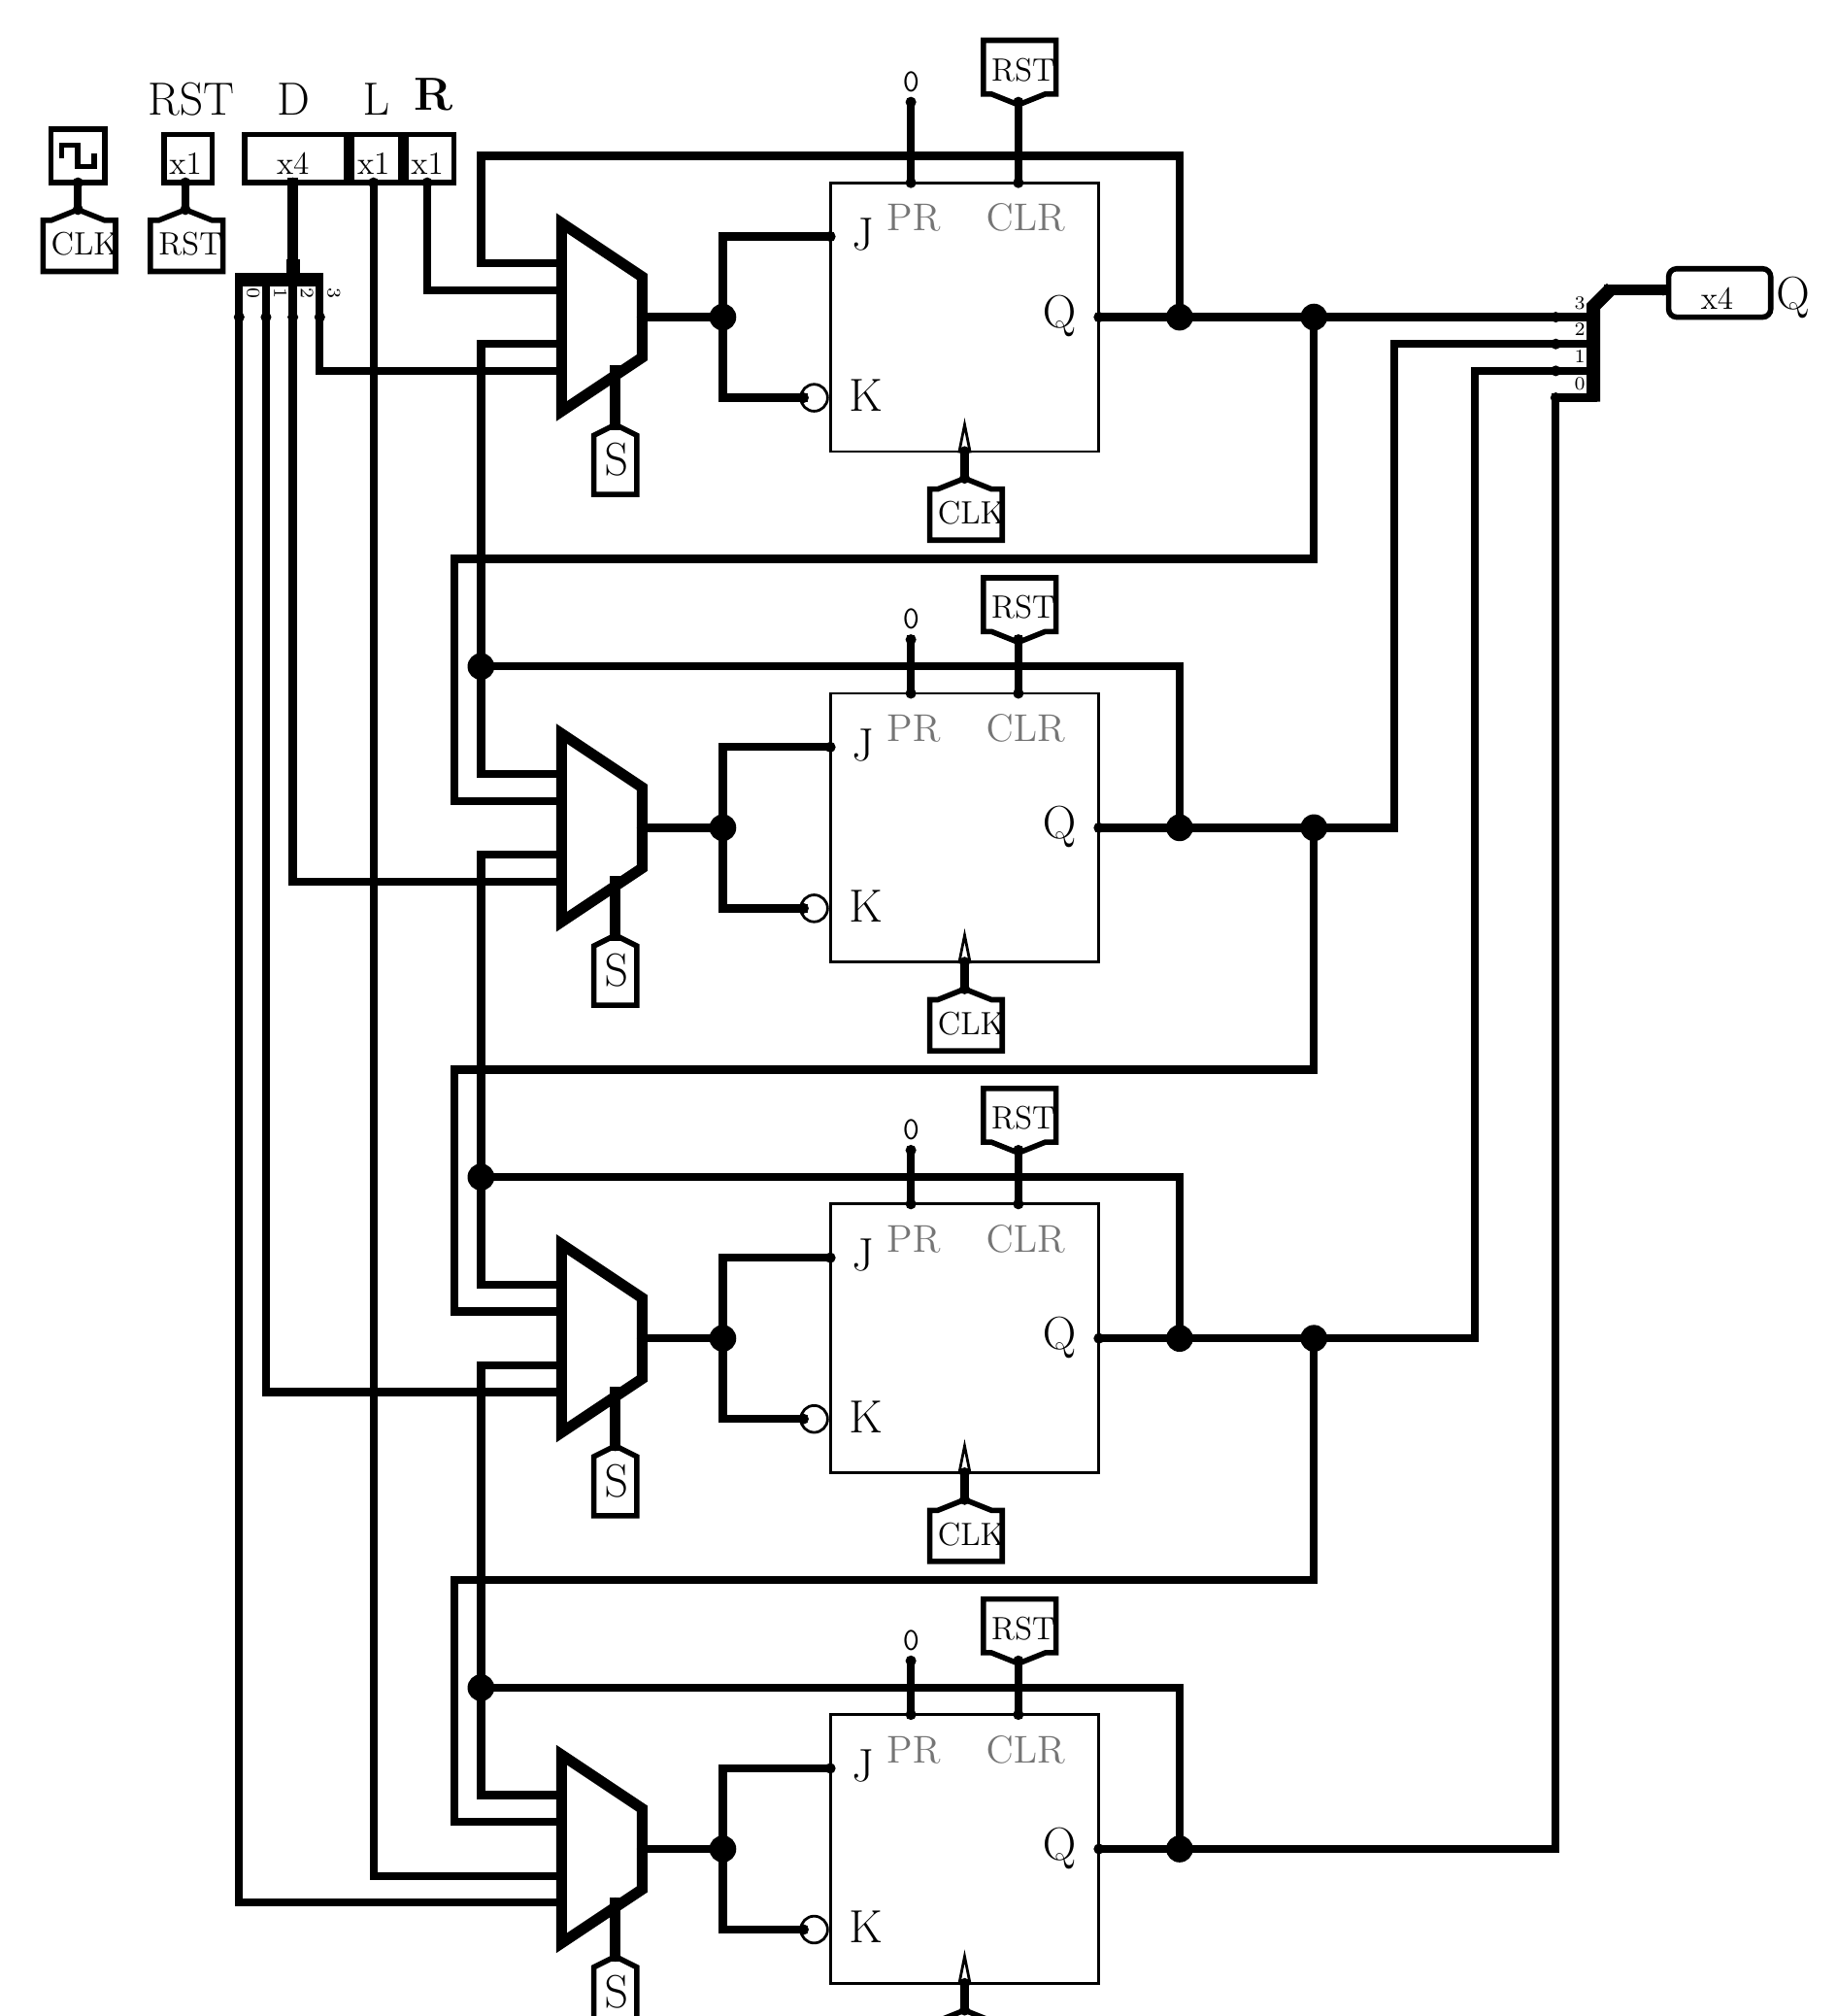
\begin{tikzpicture}[x=1pt,y=-1pt,line cap=rect]
\def\logisimfontA#1{\fontfamily{cmr}{#1}} % Replaced by logisim, original font was "SansSerif"
\def\logisimfontB#1{\fontfamily{Ubuntu}{#1}}
\def\logisimfontC#1{\fontfamily{cmtt}{#1}} % Replaced by logisim, original font was "Monospaced"
\definecolor{custcol_0_0_0}{RGB}{0, 0, 0}
\definecolor{custcol_75_75_75}{RGB}{117, 117, 117}
\definecolor{custcol_ff_ff_ff}{RGB}{255, 255, 255}
\draw [line width=3.0pt, custcol_0_0_0 ]  (349.0,538.0) -- (349.0,548.0) ;
\draw [line width=4.0pt, custcol_0_0_0 ]  (219.0,128.0) -- (219.0,148.0) ;
\draw [line width=3.0pt, custcol_0_0_0 ]  (149.0,58.0) -- (149.0,98.0) -- (199.0,98.0) ;
\draw [line width=3.0pt, custcol_0_0_0 ]  (19.0,58.0) -- (19.0,68.0) ;
\draw [line width=3.0pt, custcol_0_0_0 ]  (59.0,58.0) -- (59.0,68.0) ;
\draw [line width=3.0pt, custcol_0_0_0 ]  (349.0,348.0) -- (349.0,358.0) ;
\draw [line width=4.0pt, custcol_0_0_0 ]  (219.0,698.0) -- (219.0,718.0) ;
\draw [line width=3.0pt, custcol_0_0_0 ]  (329.0,608.0) -- (329.0,628.0) ;
\draw [line width=3.0pt, custcol_0_0_0 ]  (369.0,608.0) -- (369.0,628.0) ;
\draw [line width=4.0pt, custcol_0_0_0 ]  (99.0,58.0) -- (99.0,88.0) ;
\draw [line width=3.0pt, custcol_0_0_0 ]  (299.0,458.0) -- (259.0,458.0) -- (259.0,488.0) -- (259.0,518.0) -- (289.0,518.0) ;
\draw [line width=4.0pt, custcol_0_0_0 ]  (589.0,98.0) -- (609.0,98.0) ;
\draw [line width=3.0pt, custcol_0_0_0 ]  (229.0,488.0) -- (259.0,488.0) ;
\draw [line width=3.0pt, custcol_0_0_0 ]  (199.0,308.0) -- (169.0,308.0) -- (169.0,428.0) -- (429.0,428.0) -- (429.0,488.0) -- (399.0,488.0) ;
\draw [line width=3.0pt, custcol_0_0_0 ]  (349.0,158.0) -- (349.0,168.0) ;
\draw [line width=4.0pt, custcol_0_0_0 ]  (219.0,508.0) -- (219.0,528.0) ;
\draw [line width=3.0pt, custcol_0_0_0 ]  (329.0,418.0) -- (329.0,438.0) ;
\draw [line width=3.0pt, custcol_0_0_0 ]  (369.0,418.0) -- (369.0,438.0) ;
\draw [line width=3.0pt, custcol_0_0_0 ]  (299.0,268.0) -- (259.0,268.0) -- (259.0,298.0) -- (259.0,328.0) -- (289.0,328.0) ;
\draw [line width=3.0pt, custcol_0_0_0 ]  (169.0,238.0) -- (169.0,118.0) -- (199.0,118.0) ;
\draw [line width=3.0pt, custcol_0_0_0 ]  (229.0,298.0) -- (259.0,298.0) ;
\draw [line width=3.0pt, custcol_0_0_0 ]  (399.0,108.0) -- (429.0,108.0) -- (479.0,108.0) -- (479.0,198.0) -- (159.0,198.0) -- (159.0,288.0) -- (199.0,288.0) ;
\draw [line width=3.0pt, custcol_0_0_0 ]  (199.0,278.0) -- (169.0,278.0) -- (169.0,238.0) -- (429.0,238.0) -- (429.0,298.0) ;
\draw [line width=3.0pt, custcol_0_0_0 ]  (199.0,478.0) -- (159.0,478.0) -- (159.0,388.0) -- (479.0,388.0) -- (479.0,298.0) -- (429.0,298.0) -- (399.0,298.0) ;
\draw [line width=3.0pt, custcol_0_0_0 ]  (349.0,728.0) -- (349.0,738.0) ;
\draw [line width=4.0pt, custcol_0_0_0 ]  (219.0,318.0) -- (219.0,338.0) ;
\draw [line width=3.0pt, custcol_0_0_0 ]  (329.0,228.0) -- (329.0,248.0) ;
\draw [line width=3.0pt, custcol_0_0_0 ]  (369.0,228.0) -- (369.0,248.0) ;
\draw [line width=3.0pt, custcol_0_0_0 ]  (259.0,678.0) -- (259.0,708.0) -- (289.0,708.0) ;
\draw [line width=3.0pt, custcol_0_0_0 ]  (329.0,28.0) -- (329.0,58.0) ;
\draw [line width=3.0pt, custcol_0_0_0 ]  (369.0,28.0) -- (369.0,58.0) ;
\draw [line width=3.0pt, custcol_0_0_0 ]  (479.0,488.0) -- (479.0,578.0) -- (159.0,578.0) -- (159.0,668.0) -- (199.0,668.0) ;
\draw [line width=3.0pt, custcol_0_0_0 ]  (229.0,678.0) -- (259.0,678.0) -- (259.0,648.0) -- (299.0,648.0) ;
\draw [line width=3.0pt, custcol_0_0_0 ]  (229.0,108.0) -- (259.0,108.0) ;
\draw [line width=3.0pt, custcol_0_0_0 ]  (299.0,78.0) -- (259.0,78.0) -- (259.0,108.0) -- (259.0,138.0) -- (289.0,138.0) ;
\draw [line width=3.0pt, custcol_0_0_0 ]  (399.0,678.0) -- (429.0,678.0) ;
\draw [line width=3.0pt, custcol_0_0_0 ]  (169.0,428.0) -- (169.0,468.0) -- (199.0,468.0) ;
\draw [line width=3.0pt, custcol_0_0_0 ]  (199.0,88.0) -- (169.0,88.0) -- (169.0,48.0) -- (429.0,48.0) -- (429.0,108.0) ;
\draw [line width=3.0pt, custcol_0_0_0 ]  (129.0,58.0) -- (129.0,688.0) -- (199.0,688.0) ;
\draw [line width=3.0pt, custcol_0_0_0 ]  (199.0,498.0) -- (169.0,498.0) -- (169.0,618.0) ;
\fill [line width=3.0pt, custcol_0_0_0]  (429.0,298.0) ellipse (5.0 and 5.0 );
\fill [line width=3.0pt, custcol_0_0_0]  (169.0,428.0) ellipse (5.0 and 5.0 );
\fill [line width=3.0pt, custcol_0_0_0]  (479.0,298.0) ellipse (5.0 and 5.0 );
\fill [line width=3.0pt, custcol_0_0_0]  (259.0,488.0) ellipse (5.0 and 5.0 );
\fill [line width=3.0pt, custcol_0_0_0]  (429.0,108.0) ellipse (5.0 and 5.0 );
\fill [line width=3.0pt, custcol_0_0_0]  (169.0,238.0) ellipse (5.0 and 5.0 );
\fill [line width=3.0pt, custcol_0_0_0]  (479.0,108.0) ellipse (5.0 and 5.0 );
\fill [line width=3.0pt, custcol_0_0_0]  (259.0,298.0) ellipse (5.0 and 5.0 );
\fill [line width=3.0pt, custcol_0_0_0]  (429.0,678.0) ellipse (5.0 and 5.0 );
\fill [line width=3.0pt, custcol_0_0_0]  (259.0,108.0) ellipse (5.0 and 5.0 );
\fill [line width=3.0pt, custcol_0_0_0]  (429.0,488.0) ellipse (5.0 and 5.0 );
\fill [line width=3.0pt, custcol_0_0_0]  (169.0,618.0) ellipse (5.0 and 5.0 );
\fill [line width=3.0pt, custcol_0_0_0]  (479.0,488.0) ellipse (5.0 and 5.0 );
\fill [line width=3.0pt, custcol_0_0_0]  (259.0,678.0) ellipse (5.0 and 5.0 );
\draw [line width=2.0pt, custcol_0_0_0 ]  (9.0,38.0) -- (28.0,38.0) ;
\draw [line width=2.0pt, custcol_0_0_0 ]  (29.0,38.0) -- (29.0,57.0) ;
\draw [line width=2.0pt, custcol_0_0_0 ]  (29.0,58.0) -- (10.0,58.0) ;
\draw [line width=2.0pt, custcol_0_0_0 ]  (9.0,58.0) -- (9.0,39.0) ;
\draw [line width=2.0pt, custcol_0_0_0 ]  (13.0,48.0) -- (13.0,44.0) -- (19.0,44.0) -- (19.0,52.0) -- (25.0,52.0) -- (25.0,48.0) ;
\fill [line width=2.0pt, custcol_0_0_0]  (19.0,58.0) ellipse (2.0 and 2.0 );
\logisimfontB{\fontsize{12pt}{12pt}\fontseries{bx}\selectfont\node[inner sep=0, outer sep=0, custcol_0_0_0, anchor=base west] at  (9.0,85.0)  {CLK};}
\draw [line width=2.0pt, custcol_0_0_0 ]  (6.0,72.0) -- (9.0,72.0) -- (19.0,68.0) -- (29.0,72.0) -- (33.0,72.0) -- (33.0,91.0) -- (6.0,91.0) -- cycle;
\fill [line width=2.0pt, custcol_0_0_0]  (19.0,68.0) ellipse (2.0 and 2.0 );
\draw [line width=2.0pt, custcol_0_0_0 ]  (51.0,40.0) -- (68.0,40.0) ;
\draw [line width=2.0pt, custcol_0_0_0 ]  (69.0,40.0) -- (69.0,57.0) ;
\draw [line width=2.0pt, custcol_0_0_0 ]  (69.0,58.0) -- (52.0,58.0) ;
\draw [line width=2.0pt, custcol_0_0_0 ]  (51.0,58.0) -- (51.0,41.0) ;
\logisimfontA{\fontsize{12pt}{12pt}\selectfont\node[inner sep=0, outer sep=0, custcol_0_0_0, anchor=base west] at  (53.0,55.0)  {x1};}
\logisimfontB{\fontsize{16pt}{16pt}\fontseries{bx}\selectfont\node[inner sep=0, outer sep=0, custcol_0_0_0, anchor=base west] at  (45.0,33.0)  {RST};}
\fill [line width=2.0pt, custcol_0_0_0]  (59.0,58.0) ellipse (2.0 and 2.0 );
\logisimfontB{\fontsize{12pt}{12pt}\fontseries{bx}\selectfont\node[inner sep=0, outer sep=0, custcol_0_0_0, anchor=base west] at  (49.0,85.0)  {RST};}
\draw [line width=2.0pt, custcol_0_0_0 ]  (46.0,72.0) -- (49.0,72.0) -- (59.0,68.0) -- (69.0,72.0) -- (73.0,72.0) -- (73.0,91.0) -- (46.0,91.0) -- cycle;
\fill [line width=2.0pt, custcol_0_0_0]  (59.0,68.0) ellipse (2.0 and 2.0 );
\draw [line width=3.0pt, custcol_0_0_0 ]  (199.0,128.0) -- (109.0,128.0) -- (109.0,108.0) -- (109.0,94.0) ;
\draw [line width=3.0pt, custcol_0_0_0 ]  (199.0,318.0) -- (99.0,318.0) -- (99.0,108.0) -- (99.0,94.0) ;
\draw [line width=3.0pt, custcol_0_0_0 ]  (199.0,508.0) -- (89.0,508.0) -- (89.0,108.0) -- (89.0,94.0) ;
\draw [line width=3.0pt, custcol_0_0_0 ]  (199.0,698.0) -- (79.0,698.0) -- (79.0,108.0) -- (79.0,94.0) ;
\draw [line width=5.0pt, custcol_0_0_0 ]  (99.0,89.0) -- (99.0,94.0) ;
\draw [line width=5.0pt, custcol_0_0_0 ]  (108.0,94.0) -- (80.0,94.0) ;
\logisimfontA{\fontsize{7pt}{7pt}\selectfont\node[inner sep=0, outer sep=0, custcol_0_0_0, anchor=base west, rotate=-90.0] at  (112.0,97.0)  {3};}
\logisimfontA{\fontsize{7pt}{7pt}\selectfont\node[inner sep=0, outer sep=0, custcol_0_0_0, anchor=base west, rotate=-90.0] at  (102.0,97.0)  {2};}
\logisimfontA{\fontsize{7pt}{7pt}\selectfont\node[inner sep=0, outer sep=0, custcol_0_0_0, anchor=base west, rotate=-90.0] at  (92.0,97.0)  {1};}
\logisimfontA{\fontsize{7pt}{7pt}\selectfont\node[inner sep=0, outer sep=0, custcol_0_0_0, anchor=base west, rotate=-90.0] at  (82.0,97.0)  {0};}
\fill [line width=5.0pt, custcol_0_0_0]  (99.0,88.0) ellipse (2.0 and 2.0 );
\fill [line width=5.0pt, custcol_0_0_0]  (109.0,108.0) ellipse (2.0 and 2.0 );
\fill [line width=5.0pt, custcol_0_0_0]  (99.0,108.0) ellipse (2.0 and 2.0 );
\fill [line width=5.0pt, custcol_0_0_0]  (89.0,108.0) ellipse (2.0 and 2.0 );
\fill [line width=5.0pt, custcol_0_0_0]  (79.0,108.0) ellipse (2.0 and 2.0 );
\draw [line width=2.0pt, custcol_0_0_0 ]  (81.0,40.0) -- (118.0,40.0) ;
\draw [line width=2.0pt, custcol_0_0_0 ]  (119.0,40.0) -- (119.0,57.0) ;
\draw [line width=2.0pt, custcol_0_0_0 ]  (119.0,58.0) -- (82.0,58.0) ;
\draw [line width=2.0pt, custcol_0_0_0 ]  (81.0,58.0) -- (81.0,41.0) ;
\logisimfontA{\fontsize{12pt}{12pt}\selectfont\node[inner sep=0, outer sep=0, custcol_0_0_0, anchor=base west] at  (93.0,55.0)  {x4};}
\logisimfontB{\fontsize{16pt}{16pt}\fontseries{bx}\selectfont\node[inner sep=0, outer sep=0, custcol_0_0_0, anchor=base west] at  (93.0,33.0)  {D};}
\fill [line width=2.0pt, custcol_0_0_0]  (99.0,58.0) ellipse (2.0 and 2.0 );
\draw [line width=2.0pt, custcol_0_0_0 ]  (121.0,40.0) -- (138.0,40.0) ;
\draw [line width=2.0pt, custcol_0_0_0 ]  (139.0,40.0) -- (139.0,57.0) ;
\draw [line width=2.0pt, custcol_0_0_0 ]  (139.0,58.0) -- (122.0,58.0) ;
\draw [line width=2.0pt, custcol_0_0_0 ]  (121.0,58.0) -- (121.0,41.0) ;
\logisimfontA{\fontsize{12pt}{12pt}\selectfont\node[inner sep=0, outer sep=0, custcol_0_0_0, anchor=base west] at  (123.0,55.0)  {x1};}
\logisimfontB{\fontsize{16pt}{16pt}\fontseries{bx}\selectfont\node[inner sep=0, outer sep=0, custcol_0_0_0, anchor=base west] at  (125.0,33.0)  {L};}
\fill [line width=2.0pt, custcol_0_0_0]  (129.0,58.0) ellipse (2.0 and 2.0 );
\draw [line width=2.0pt, custcol_0_0_0 ]  (141.0,40.0) -- (158.0,40.0) ;
\draw [line width=2.0pt, custcol_0_0_0 ]  (159.0,40.0) -- (159.0,57.0) ;
\draw [line width=2.0pt, custcol_0_0_0 ]  (159.0,58.0) -- (142.0,58.0) ;
\draw [line width=2.0pt, custcol_0_0_0 ]  (141.0,58.0) -- (141.0,41.0) ;
\logisimfontA{\fontsize{12pt}{12pt}\selectfont\node[inner sep=0, outer sep=0, custcol_0_0_0, anchor=base west] at  (143.0,55.0)  {x1};}
\logisimfontA{\fontsize{16pt}{16pt}\fontseries{bx}\selectfont\node[inner sep=0, outer sep=0, custcol_0_0_0, anchor=base west] at  (144.0,31.0)  {R};}
\fill [line width=2.0pt, custcol_0_0_0]  (149.0,58.0) ellipse (2.0 and 2.0 );
\logisimfontB{\fontsize{16pt}{16pt}\fontseries{bx}\selectfont\node[inner sep=0, outer sep=0, custcol_0_0_0, anchor=base west] at  (215.0,167.0)  {S};}
\draw [line width=2.0pt, custcol_0_0_0 ]  (211.0,152.0) -- (219.0,148.0) -- (227.0,152.0) -- (227.0,174.0) -- (211.0,174.0) -- cycle;
\fill [line width=2.0pt, custcol_0_0_0]  (219.0,148.0) ellipse (2.0 and 2.0 );
\logisimfontB{\fontsize{16pt}{16pt}\fontseries{bx}\selectfont\node[inner sep=0, outer sep=0, custcol_0_0_0, anchor=base west] at  (215.0,357.0)  {S};}
\draw [line width=2.0pt, custcol_0_0_0 ]  (211.0,342.0) -- (219.0,338.0) -- (227.0,342.0) -- (227.0,364.0) -- (211.0,364.0) -- cycle;
\fill [line width=2.0pt, custcol_0_0_0]  (219.0,338.0) ellipse (2.0 and 2.0 );
\logisimfontB{\fontsize{16pt}{16pt}\fontseries{bx}\selectfont\node[inner sep=0, outer sep=0, custcol_0_0_0, anchor=base west] at  (215.0,547.0)  {S};}
\draw [line width=2.0pt, custcol_0_0_0 ]  (211.0,532.0) -- (219.0,528.0) -- (227.0,532.0) -- (227.0,554.0) -- (211.0,554.0) -- cycle;
\fill [line width=2.0pt, custcol_0_0_0]  (219.0,528.0) ellipse (2.0 and 2.0 );
\logisimfontB{\fontsize{16pt}{16pt}\fontseries{bx}\selectfont\node[inner sep=0, outer sep=0, custcol_0_0_0, anchor=base west] at  (215.0,737.0)  {S};}
\draw [line width=2.0pt, custcol_0_0_0 ]  (211.0,722.0) -- (219.0,718.0) -- (227.0,722.0) -- (227.0,744.0) -- (211.0,744.0) -- cycle;
\fill [line width=2.0pt, custcol_0_0_0]  (219.0,718.0) ellipse (2.0 and 2.0 );
\logisimfontC{\fontsize{12pt}{12pt}\selectfont\node[inner sep=0, outer sep=0, custcol_0_0_0, anchor=base west] at  (326.0,224.0)  {0};}
\fill [line width=1.0pt, custcol_0_0_0]  (329.0,228.0) ellipse (2.0 and 2.0 );
\logisimfontC{\fontsize{12pt}{12pt}\selectfont\node[inner sep=0, outer sep=0, custcol_0_0_0, anchor=base west] at  (326.0,414.0)  {0};}
\fill [line width=1.0pt, custcol_0_0_0]  (329.0,418.0) ellipse (2.0 and 2.0 );
\logisimfontC{\fontsize{12pt}{12pt}\selectfont\node[inner sep=0, outer sep=0, custcol_0_0_0, anchor=base west] at  (326.0,24.0)  {0};}
\fill [line width=1.0pt, custcol_0_0_0]  (329.0,28.0) ellipse (2.0 and 2.0 );
\logisimfontC{\fontsize{12pt}{12pt}\selectfont\node[inner sep=0, outer sep=0, custcol_0_0_0, anchor=base west] at  (326.0,604.0)  {0};}
\fill [line width=1.0pt, custcol_0_0_0]  (329.0,608.0) ellipse (2.0 and 2.0 );
\logisimfontB{\fontsize{12pt}{12pt}\fontseries{bx}\selectfont\node[inner sep=0, outer sep=0, custcol_0_0_0, anchor=base west] at  (339.0,185.0)  {CLK};}
\draw [line width=2.0pt, custcol_0_0_0 ]  (336.0,172.0) -- (339.0,172.0) -- (349.0,168.0) -- (359.0,172.0) -- (363.0,172.0) -- (363.0,191.0) -- (336.0,191.0) -- cycle;
\fill [line width=2.0pt, custcol_0_0_0]  (349.0,168.0) ellipse (2.0 and 2.0 );
\logisimfontB{\fontsize{12pt}{12pt}\fontseries{bx}\selectfont\node[inner sep=0, outer sep=0, custcol_0_0_0, anchor=base west] at  (339.0,375.0)  {CLK};}
\draw [line width=2.0pt, custcol_0_0_0 ]  (336.0,362.0) -- (339.0,362.0) -- (349.0,358.0) -- (359.0,362.0) -- (363.0,362.0) -- (363.0,381.0) -- (336.0,381.0) -- cycle;
\fill [line width=2.0pt, custcol_0_0_0]  (349.0,358.0) ellipse (2.0 and 2.0 );
\logisimfontB{\fontsize{12pt}{12pt}\fontseries{bx}\selectfont\node[inner sep=0, outer sep=0, custcol_0_0_0, anchor=base west] at  (339.0,565.0)  {CLK};}
\draw [line width=2.0pt, custcol_0_0_0 ]  (336.0,552.0) -- (339.0,552.0) -- (349.0,548.0) -- (359.0,552.0) -- (363.0,552.0) -- (363.0,571.0) -- (336.0,571.0) -- cycle;
\fill [line width=2.0pt, custcol_0_0_0]  (349.0,548.0) ellipse (2.0 and 2.0 );
\logisimfontB{\fontsize{12pt}{12pt}\fontseries{bx}\selectfont\node[inner sep=0, outer sep=0, custcol_0_0_0, anchor=base west] at  (339.0,755.0)  {CLK};}
\draw [line width=2.0pt, custcol_0_0_0 ]  (336.0,742.0) -- (339.0,742.0) -- (349.0,738.0) -- (359.0,742.0) -- (363.0,742.0) -- (363.0,761.0) -- (336.0,761.0) -- cycle;
\fill [line width=2.0pt, custcol_0_0_0]  (349.0,738.0) ellipse (2.0 and 2.0 );
\logisimfontB{\fontsize{12pt}{12pt}\fontseries{bx}\selectfont\node[inner sep=0, outer sep=0, custcol_0_0_0, anchor=base west] at  (359.0,220.0)  {RST};}
\draw [line width=2.0pt, custcol_0_0_0 ]  (356.0,205.0) -- (383.0,205.0) -- (383.0,225.0) -- (379.0,225.0) -- (369.0,229.0) -- (359.0,225.0) -- (356.0,225.0) -- cycle;
\fill [line width=2.0pt, custcol_0_0_0]  (369.0,228.0) ellipse (2.0 and 2.0 );
\logisimfontB{\fontsize{12pt}{12pt}\fontseries{bx}\selectfont\node[inner sep=0, outer sep=0, custcol_0_0_0, anchor=base west] at  (359.0,410.0)  {RST};}
\draw [line width=2.0pt, custcol_0_0_0 ]  (356.0,395.0) -- (383.0,395.0) -- (383.0,415.0) -- (379.0,415.0) -- (369.0,419.0) -- (359.0,415.0) -- (356.0,415.0) -- cycle;
\fill [line width=2.0pt, custcol_0_0_0]  (369.0,418.0) ellipse (2.0 and 2.0 );
\logisimfontB{\fontsize{12pt}{12pt}\fontseries{bx}\selectfont\node[inner sep=0, outer sep=0, custcol_0_0_0, anchor=base west] at  (359.0,20.0)  {RST};}
\draw [line width=2.0pt, custcol_0_0_0 ]  (356.0,5.0) -- (383.0,5.0) -- (383.0,25.0) -- (379.0,25.0) -- (369.0,29.0) -- (359.0,25.0) -- (356.0,25.0) -- cycle;
\fill [line width=2.0pt, custcol_0_0_0]  (369.0,28.0) ellipse (2.0 and 2.0 );
\logisimfontB{\fontsize{12pt}{12pt}\fontseries{bx}\selectfont\node[inner sep=0, outer sep=0, custcol_0_0_0, anchor=base west] at  (359.0,600.0)  {RST};}
\draw [line width=2.0pt, custcol_0_0_0 ]  (356.0,585.0) -- (383.0,585.0) -- (383.0,605.0) -- (379.0,605.0) -- (369.0,609.0) -- (359.0,605.0) -- (356.0,605.0) -- cycle;
\fill [line width=2.0pt, custcol_0_0_0]  (369.0,608.0) ellipse (2.0 and 2.0 );
\draw [line width=3.0pt, custcol_0_0_0 ]  (479.0,108.0) -- (569.0,108.0) -- (583.0,108.0) ;
\draw [line width=3.0pt, custcol_0_0_0 ]  (479.0,298.0) -- (509.0,298.0) -- (509.0,118.0) -- (569.0,118.0) -- (583.0,118.0) ;
\draw [line width=3.0pt, custcol_0_0_0 ]  (429.0,488.0) -- (479.0,488.0) -- (539.0,488.0) -- (539.0,128.0) -- (569.0,128.0) -- (583.0,128.0) ;
\draw [line width=3.0pt, custcol_0_0_0 ]  (199.0,658.0) -- (169.0,658.0) -- (169.0,618.0) -- (429.0,618.0) -- (429.0,678.0) -- (569.0,678.0) -- (569.0,138.0) -- (583.0,138.0) ;
\draw [line width=5.0pt, custcol_0_0_0 ]  (583.0,137.0) -- (583.0,104.0) -- (588.0,99.0) ;
\logisimfontA{\fontsize{7pt}{7pt}\selectfont\node[inner sep=0, outer sep=0, custcol_0_0_0, anchor=base west] at  (576.0,105.0)  {3};}
\logisimfontA{\fontsize{7pt}{7pt}\selectfont\node[inner sep=0, outer sep=0, custcol_0_0_0, anchor=base west] at  (576.0,115.0)  {2};}
\logisimfontA{\fontsize{7pt}{7pt}\selectfont\node[inner sep=0, outer sep=0, custcol_0_0_0, anchor=base west] at  (576.0,125.0)  {1};}
\logisimfontA{\fontsize{7pt}{7pt}\selectfont\node[inner sep=0, outer sep=0, custcol_0_0_0, anchor=base west] at  (576.0,135.0)  {0};}
\fill [line width=5.0pt, custcol_0_0_0]  (589.0,98.0) ellipse (2.0 and 2.0 );
\fill [line width=5.0pt, custcol_0_0_0]  (569.0,108.0) ellipse (2.0 and 2.0 );
\fill [line width=5.0pt, custcol_0_0_0]  (569.0,118.0) ellipse (2.0 and 2.0 );
\fill [line width=5.0pt, custcol_0_0_0]  (569.0,128.0) ellipse (2.0 and 2.0 );
\fill [line width=5.0pt, custcol_0_0_0]  (569.0,138.0) ellipse (2.0 and 2.0 );
\begin{pgfpicture}
   \begin{pgfmagnify}{1pt}{-1pt}
      \pgfsetrectcap
      \pgfsetcornersarced{\pgfpoint{3.0}{3.0}}
      \pgfsetlinewidth{2.0}
      \color{custcol_0_0_0}
      \pgfsetfillopacity{1.0}
      \pgfpathrectanglecorners{\pgfpoint{611.0}{90.0}}{\pgfpoint{649.0}{108.0}}
      \pgfusepath{stroke}
   \end{pgfmagnify}
\end{pgfpicture}
\logisimfontA{\fontsize{12pt}{12pt}\selectfont\node[inner sep=0, outer sep=0, custcol_0_0_0, anchor=base west] at  (623.0,105.0)  {x4};}
\logisimfontB{\fontsize{16pt}{16pt}\fontseries{bx}\selectfont\node[inner sep=0, outer sep=0, custcol_0_0_0, anchor=base west] at  (651.0,105.0)  {Q};}
\fill [line width=2.0pt, custcol_0_0_0]  (609.0,98.0) ellipse (2.0 and 2.0 );
\draw [line width=4.0pt, custcol_0_0_0 ]  (199.0,73.0) -- (199.0,143.0) -- (229.0,123.0) -- (229.0,93.0) -- cycle;
\fill [line width=1.0pt, custcol_0_0_0]  (199.0,88.0) ellipse (2.0 and 2.0 );
\fill [line width=1.0pt, custcol_0_0_0]  (199.0,98.0) ellipse (2.0 and 2.0 );
\fill [line width=1.0pt, custcol_0_0_0]  (199.0,118.0) ellipse (2.0 and 2.0 );
\fill [line width=1.0pt, custcol_0_0_0]  (199.0,128.0) ellipse (2.0 and 2.0 );
\fill [line width=1.0pt, custcol_0_0_0]  (219.0,128.0) ellipse (2.0 and 2.0 );
\fill [line width=1.0pt, custcol_0_0_0]  (229.0,108.0) ellipse (2.0 and 2.0 );
\draw [line width=4.0pt, custcol_0_0_0 ]  (199.0,263.0) -- (199.0,333.0) -- (229.0,313.0) -- (229.0,283.0) -- cycle;
\fill [line width=1.0pt, custcol_0_0_0]  (199.0,278.0) ellipse (2.0 and 2.0 );
\fill [line width=1.0pt, custcol_0_0_0]  (199.0,288.0) ellipse (2.0 and 2.0 );
\fill [line width=1.0pt, custcol_0_0_0]  (199.0,308.0) ellipse (2.0 and 2.0 );
\fill [line width=1.0pt, custcol_0_0_0]  (199.0,318.0) ellipse (2.0 and 2.0 );
\fill [line width=1.0pt, custcol_0_0_0]  (219.0,318.0) ellipse (2.0 and 2.0 );
\fill [line width=1.0pt, custcol_0_0_0]  (229.0,298.0) ellipse (2.0 and 2.0 );
\draw [line width=4.0pt, custcol_0_0_0 ]  (199.0,453.0) -- (199.0,523.0) -- (229.0,503.0) -- (229.0,473.0) -- cycle;
\fill [line width=1.0pt, custcol_0_0_0]  (199.0,468.0) ellipse (2.0 and 2.0 );
\fill [line width=1.0pt, custcol_0_0_0]  (199.0,478.0) ellipse (2.0 and 2.0 );
\fill [line width=1.0pt, custcol_0_0_0]  (199.0,498.0) ellipse (2.0 and 2.0 );
\fill [line width=1.0pt, custcol_0_0_0]  (199.0,508.0) ellipse (2.0 and 2.0 );
\fill [line width=1.0pt, custcol_0_0_0]  (219.0,508.0) ellipse (2.0 and 2.0 );
\fill [line width=1.0pt, custcol_0_0_0]  (229.0,488.0) ellipse (2.0 and 2.0 );
\draw [line width=4.0pt, custcol_0_0_0 ]  (199.0,643.0) -- (199.0,713.0) -- (229.0,693.0) -- (229.0,663.0) -- cycle;
\fill [line width=1.0pt, custcol_0_0_0]  (199.0,658.0) ellipse (2.0 and 2.0 );
\fill [line width=1.0pt, custcol_0_0_0]  (199.0,668.0) ellipse (2.0 and 2.0 );
\fill [line width=1.0pt, custcol_0_0_0]  (199.0,688.0) ellipse (2.0 and 2.0 );
\fill [line width=1.0pt, custcol_0_0_0]  (199.0,698.0) ellipse (2.0 and 2.0 );
\fill [line width=1.0pt, custcol_0_0_0]  (219.0,698.0) ellipse (2.0 and 2.0 );
\fill [line width=1.0pt, custcol_0_0_0]  (229.0,678.0) ellipse (2.0 and 2.0 );
\draw [line width=1.0pt, custcol_0_0_0 ]  (299.0,58.0) -- (398.0,58.0) ;
\draw [line width=1.0pt, custcol_0_0_0 ]  (399.0,58.0) -- (399.0,157.0) ;
\draw [line width=1.0pt, custcol_0_0_0 ]  (399.0,158.0) -- (300.0,158.0) ;
\draw [line width=1.0pt, custcol_0_0_0 ]  (299.0,158.0) -- (299.0,59.0) ;
\draw [line width=1.0pt, custcol_0_0_0 ]  (349.0,148.0) -- (347.0,158.0) -- (351.0,158.0) -- cycle;
\logisimfontB{\fontsize{16pt}{16pt}\fontseries{bx}\selectfont\node[inner sep=0, outer sep=0, custcol_0_0_0, anchor=base west] at  (307.0,83.0)  {J};}
\logisimfontB{\fontsize{16pt}{16pt}\fontseries{bx}\selectfont\node[inner sep=0, outer sep=0, custcol_0_0_0, anchor=base west] at  (306.0,143.0)  {K};}
\logisimfontB{\fontsize{16pt}{16pt}\fontseries{bx}\selectfont\node[inner sep=0, outer sep=0, custcol_0_0_0, anchor=base west] at  (378.0,112.0)  {Q};}
\logisimfontB{\fontsize{14pt}{14pt}\fontseries{bx}\selectfont\node[inner sep=0, outer sep=0, custcol_75_75_75, anchor=base west] at  (320.0,76.0)  {PR};}
\logisimfontB{\fontsize{14pt}{14pt}\fontseries{bx}\selectfont\node[inner sep=0, outer sep=0, custcol_75_75_75, anchor=base west] at  (357.0,76.0)  {CLR};}
\draw [line width=1.0pt, custcol_0_0_0]  (293.0,138.0) ellipse (5.0 and 5.0 );
\fill [line width=1.0pt, custcol_0_0_0]  (289.0,138.0) ellipse (2.0 and 2.0 );
\fill [line width=1.0pt, custcol_0_0_0]  (299.0,78.0) ellipse (2.0 and 2.0 );
\fill [line width=1.0pt, custcol_0_0_0]  (329.0,58.0) ellipse (2.0 and 2.0 );
\fill [line width=1.0pt, custcol_0_0_0]  (349.0,158.0) ellipse (2.0 and 2.0 );
\fill [line width=1.0pt, custcol_0_0_0]  (369.0,58.0) ellipse (2.0 and 2.0 );
\fill [line width=1.0pt, custcol_0_0_0]  (399.0,108.0) ellipse (2.0 and 2.0 );
\draw [line width=1.0pt, custcol_0_0_0 ]  (299.0,248.0) -- (398.0,248.0) ;
\draw [line width=1.0pt, custcol_0_0_0 ]  (399.0,248.0) -- (399.0,347.0) ;
\draw [line width=1.0pt, custcol_0_0_0 ]  (399.0,348.0) -- (300.0,348.0) ;
\draw [line width=1.0pt, custcol_0_0_0 ]  (299.0,348.0) -- (299.0,249.0) ;
\draw [line width=1.0pt, custcol_0_0_0 ]  (349.0,338.0) -- (347.0,348.0) -- (351.0,348.0) -- cycle;
\logisimfontB{\fontsize{16pt}{16pt}\fontseries{bx}\selectfont\node[inner sep=0, outer sep=0, custcol_0_0_0, anchor=base west] at  (307.0,273.0)  {J};}
\logisimfontB{\fontsize{16pt}{16pt}\fontseries{bx}\selectfont\node[inner sep=0, outer sep=0, custcol_0_0_0, anchor=base west] at  (306.0,333.0)  {K};}
\logisimfontB{\fontsize{16pt}{16pt}\fontseries{bx}\selectfont\node[inner sep=0, outer sep=0, custcol_0_0_0, anchor=base west] at  (378.0,302.0)  {Q};}
\logisimfontB{\fontsize{14pt}{14pt}\fontseries{bx}\selectfont\node[inner sep=0, outer sep=0, custcol_75_75_75, anchor=base west] at  (320.0,266.0)  {PR};}
\logisimfontB{\fontsize{14pt}{14pt}\fontseries{bx}\selectfont\node[inner sep=0, outer sep=0, custcol_75_75_75, anchor=base west] at  (357.0,266.0)  {CLR};}
\draw [line width=1.0pt, custcol_0_0_0]  (293.0,328.0) ellipse (5.0 and 5.0 );
\fill [line width=1.0pt, custcol_0_0_0]  (289.0,328.0) ellipse (2.0 and 2.0 );
\fill [line width=1.0pt, custcol_0_0_0]  (299.0,268.0) ellipse (2.0 and 2.0 );
\fill [line width=1.0pt, custcol_0_0_0]  (329.0,248.0) ellipse (2.0 and 2.0 );
\fill [line width=1.0pt, custcol_0_0_0]  (349.0,348.0) ellipse (2.0 and 2.0 );
\fill [line width=1.0pt, custcol_0_0_0]  (369.0,248.0) ellipse (2.0 and 2.0 );
\fill [line width=1.0pt, custcol_0_0_0]  (399.0,298.0) ellipse (2.0 and 2.0 );
\draw [line width=1.0pt, custcol_0_0_0 ]  (299.0,438.0) -- (398.0,438.0) ;
\draw [line width=1.0pt, custcol_0_0_0 ]  (399.0,438.0) -- (399.0,537.0) ;
\draw [line width=1.0pt, custcol_0_0_0 ]  (399.0,538.0) -- (300.0,538.0) ;
\draw [line width=1.0pt, custcol_0_0_0 ]  (299.0,538.0) -- (299.0,439.0) ;
\draw [line width=1.0pt, custcol_0_0_0 ]  (349.0,528.0) -- (347.0,538.0) -- (351.0,538.0) -- cycle;
\logisimfontB{\fontsize{16pt}{16pt}\fontseries{bx}\selectfont\node[inner sep=0, outer sep=0, custcol_0_0_0, anchor=base west] at  (307.0,463.0)  {J};}
\logisimfontB{\fontsize{16pt}{16pt}\fontseries{bx}\selectfont\node[inner sep=0, outer sep=0, custcol_0_0_0, anchor=base west] at  (306.0,523.0)  {K};}
\logisimfontB{\fontsize{16pt}{16pt}\fontseries{bx}\selectfont\node[inner sep=0, outer sep=0, custcol_0_0_0, anchor=base west] at  (378.0,492.0)  {Q};}
\logisimfontB{\fontsize{14pt}{14pt}\fontseries{bx}\selectfont\node[inner sep=0, outer sep=0, custcol_75_75_75, anchor=base west] at  (320.0,456.0)  {PR};}
\logisimfontB{\fontsize{14pt}{14pt}\fontseries{bx}\selectfont\node[inner sep=0, outer sep=0, custcol_75_75_75, anchor=base west] at  (357.0,456.0)  {CLR};}
\draw [line width=1.0pt, custcol_0_0_0]  (293.0,518.0) ellipse (5.0 and 5.0 );
\fill [line width=1.0pt, custcol_0_0_0]  (289.0,518.0) ellipse (2.0 and 2.0 );
\fill [line width=1.0pt, custcol_0_0_0]  (299.0,458.0) ellipse (2.0 and 2.0 );
\fill [line width=1.0pt, custcol_0_0_0]  (329.0,438.0) ellipse (2.0 and 2.0 );
\fill [line width=1.0pt, custcol_0_0_0]  (349.0,538.0) ellipse (2.0 and 2.0 );
\fill [line width=1.0pt, custcol_0_0_0]  (369.0,438.0) ellipse (2.0 and 2.0 );
\fill [line width=1.0pt, custcol_0_0_0]  (399.0,488.0) ellipse (2.0 and 2.0 );
\draw [line width=1.0pt, custcol_0_0_0 ]  (299.0,628.0) -- (398.0,628.0) ;
\draw [line width=1.0pt, custcol_0_0_0 ]  (399.0,628.0) -- (399.0,727.0) ;
\draw [line width=1.0pt, custcol_0_0_0 ]  (399.0,728.0) -- (300.0,728.0) ;
\draw [line width=1.0pt, custcol_0_0_0 ]  (299.0,728.0) -- (299.0,629.0) ;
\draw [line width=1.0pt, custcol_0_0_0 ]  (349.0,718.0) -- (347.0,728.0) -- (351.0,728.0) -- cycle;
\logisimfontB{\fontsize{16pt}{16pt}\fontseries{bx}\selectfont\node[inner sep=0, outer sep=0, custcol_0_0_0, anchor=base west] at  (307.0,653.0)  {J};}
\logisimfontB{\fontsize{16pt}{16pt}\fontseries{bx}\selectfont\node[inner sep=0, outer sep=0, custcol_0_0_0, anchor=base west] at  (306.0,713.0)  {K};}
\logisimfontB{\fontsize{16pt}{16pt}\fontseries{bx}\selectfont\node[inner sep=0, outer sep=0, custcol_0_0_0, anchor=base west] at  (378.0,682.0)  {Q};}
\logisimfontB{\fontsize{14pt}{14pt}\fontseries{bx}\selectfont\node[inner sep=0, outer sep=0, custcol_75_75_75, anchor=base west] at  (320.0,646.0)  {PR};}
\logisimfontB{\fontsize{14pt}{14pt}\fontseries{bx}\selectfont\node[inner sep=0, outer sep=0, custcol_75_75_75, anchor=base west] at  (357.0,646.0)  {CLR};}
\draw [line width=1.0pt, custcol_0_0_0]  (293.0,708.0) ellipse (5.0 and 5.0 );
\fill [line width=1.0pt, custcol_0_0_0]  (289.0,708.0) ellipse (2.0 and 2.0 );
\fill [line width=1.0pt, custcol_0_0_0]  (299.0,648.0) ellipse (2.0 and 2.0 );
\fill [line width=1.0pt, custcol_0_0_0]  (329.0,628.0) ellipse (2.0 and 2.0 );
\fill [line width=1.0pt, custcol_0_0_0]  (349.0,728.0) ellipse (2.0 and 2.0 );
\fill [line width=1.0pt, custcol_0_0_0]  (369.0,628.0) ellipse (2.0 and 2.0 );
\fill [line width=1.0pt, custcol_0_0_0]  (399.0,678.0) ellipse (2.0 and 2.0 );
\end{tikzpicture}

